\section{実験結果}

\subsection{引張試験}
表\ref{tbl:試験片寸法}に各実験条件で用いた試験片の寸法を示す.
\begin{table}[htbp]
  \centering
    \caption{Specimen width and thickness.}
    \label{tbl:試験片寸法}
    \scalebox{1}{
  \begin{tabular}{ccc}
  \hline
       & 幅h{[}mm{]} & 厚さt{[}mm{]} \\ \hline
  急冷   & 3.90        & 0.832       \\ \hline
  65$^\circ$C  & 3.91       & 0.867       \\ \hline
  120$^\circ$C  & 3.91       & 0.866       \\ \hline
  \end{tabular}
    }    
\end{table}

図\ref{fig:SS-rapid},図\ref{fig:SS-65},図\ref{fig:SS-120}にそれぞれ急冷,65$^\circ$Cで10分間保持,120$^\circ$Cで10分間保持したときの応力-ひずみ線図を示す.

本実験では,応力とひずみをカメラで測定する方法と試験機側で測定する方法の2種類を用いた.試験機で測定した結果には,試験機のツメや試験片の標線外の伸びによる誤差が含まれるため,カメラで測定した結果の方が正確である.しかし,カメラでは測定可能範囲が限られるため,測定範囲を超える領域は試験機側の測定結果で補う必要がある.
\clearpage

図\ref{fig:SS-rapid}ではひずみが1.97となる点までをカメラによるグラフにし,そこから試験機で測定したグラフを接続した.図\ref{fig:SS-65}では,ひずみが2.02となる点から試験機で測定したグラフを接続した.図\ref{fig:SS-120}ではカメラの測定範囲内で破断したため,グラフの接続は行っていない.
図\ref{fig:SS-rapid}より,急冷した試験片では34MPaあたりで降伏した後,応力が一度減少し,その後大きく伸びながら応力が上昇していくのが分かる.破断時には応力50MPa,ひずみ25程度にまで達している.図\ref{fig:SS-65}より,65$^\circ$Cで保持した試験片では急冷したときよりも高い応力で降伏し,同様に一度応力が下がってからひずみが増加し始めるが,急冷のときよりも早く破断したことが分かる.破断時の応力は約33MPa,ひずみは11程度であった.図\ref{fig:SS-120}より,120$^\circ$Cで保持した試験片でも急冷したときよりも高い応力で降伏するが,その後あまりひずみが増加せずに応力がやや減少し,すぐに破断に至っている.破断時の応力は約33MPa,ひずみは0.2程度であった.
\begin{figure}
  \centering %中央揃え
  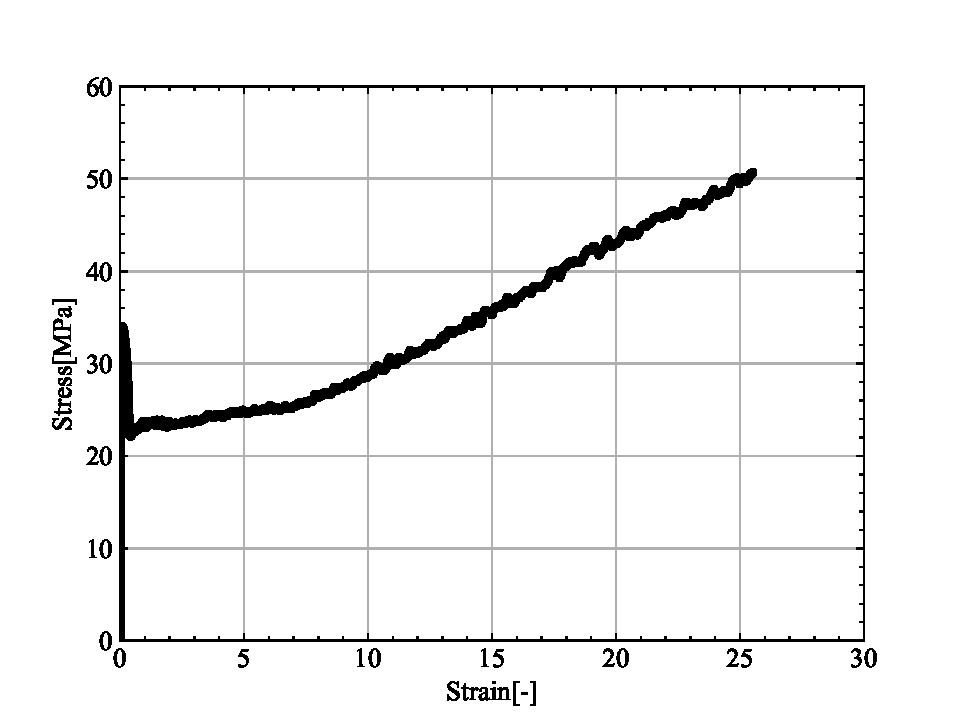
\includegraphics[width=100truemm,clip]{fig/fig_SS-rapid.pdf}
  \caption{Stress-strain diagram (rapid cooling).}
  \label{fig:SS-rapid}
\end{figure}
\begin{figure}[htbp]
  \centering %中央揃え
  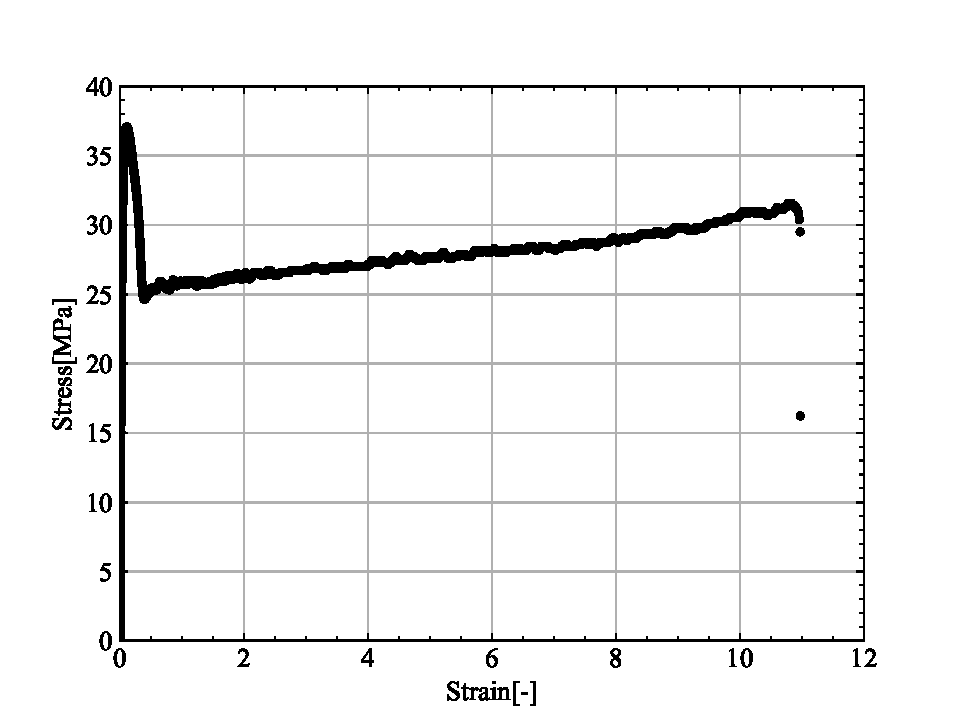
\includegraphics[width=100truemm,clip]{fig/fig_SS-65.pdf}
  \caption{Stress-strain diagram (held at 65$^\circ$C).}
  \label{fig:SS-65}
\end{figure}
\begin{figure}[htbp]
  \centering %中央揃え
  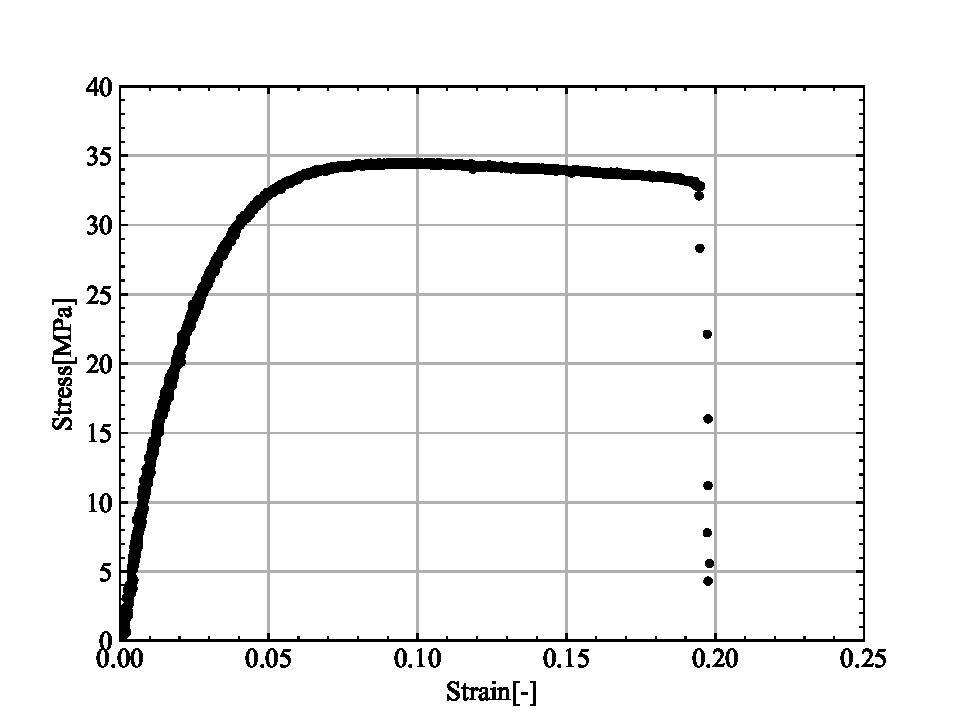
\includegraphics[width=100truemm,clip]{fig/fig_SS-120.pdf}
  \caption{Stress-strain diagram (held at 120$^\circ$C).}
  \label{fig:SS-120}
\end{figure}

表\ref{tbl:物性値}に各試験片におけるヤング率と降伏応力を示す.ヤング率は応力が0から20MPaとなる範囲での傾きから算出した.ヤング率は急冷が最も高く,降伏応力は65$^\circ$Cで保持したときが最も高いという結果となった
\begin{table}[htbp]
  \centering
    \caption{Mechanical properties of each specimen.}
    \label{tbl:物性値}
    \scalebox{1}{
  \begin{tabular}{ccc}
  \hline
       & ヤング率{[}GPa{]} & 降伏応力{[}MPa{]} \\ \hline
  急冷   & 1.16          & 34.0          \\ \hline
  65度  & 1.09          & 37.1          \\ \hline
  120度 & 1.07          & 34.5          \\ \hline
  \end{tabular}
    }
\end{table}

\subsection{組織観察結果}
図\ref{fig:rapid}に急冷したときの組織観察結果を倍率200倍と500倍で示す.同様に65$^\circ$Cで10分間保持したときの結果を図\ref{fig:65度}に,120$^\circ$Cで10分間保持したときの結果を図\ref{fig:120度}に示す.

図\ref{fig:rapid}では球晶がほとんどみられないが,図\ref{fig:65度}では小さい球晶が成長しており,直径は約30$\mu$m程度である.図\ref{fig:120度}では球晶が大きく成長しており,直径は約100$\mu$m程度になっている.
\begin{figure}[htbp]
    \begin{minipage}[htbp]{0.45\linewidth}
      \centering
      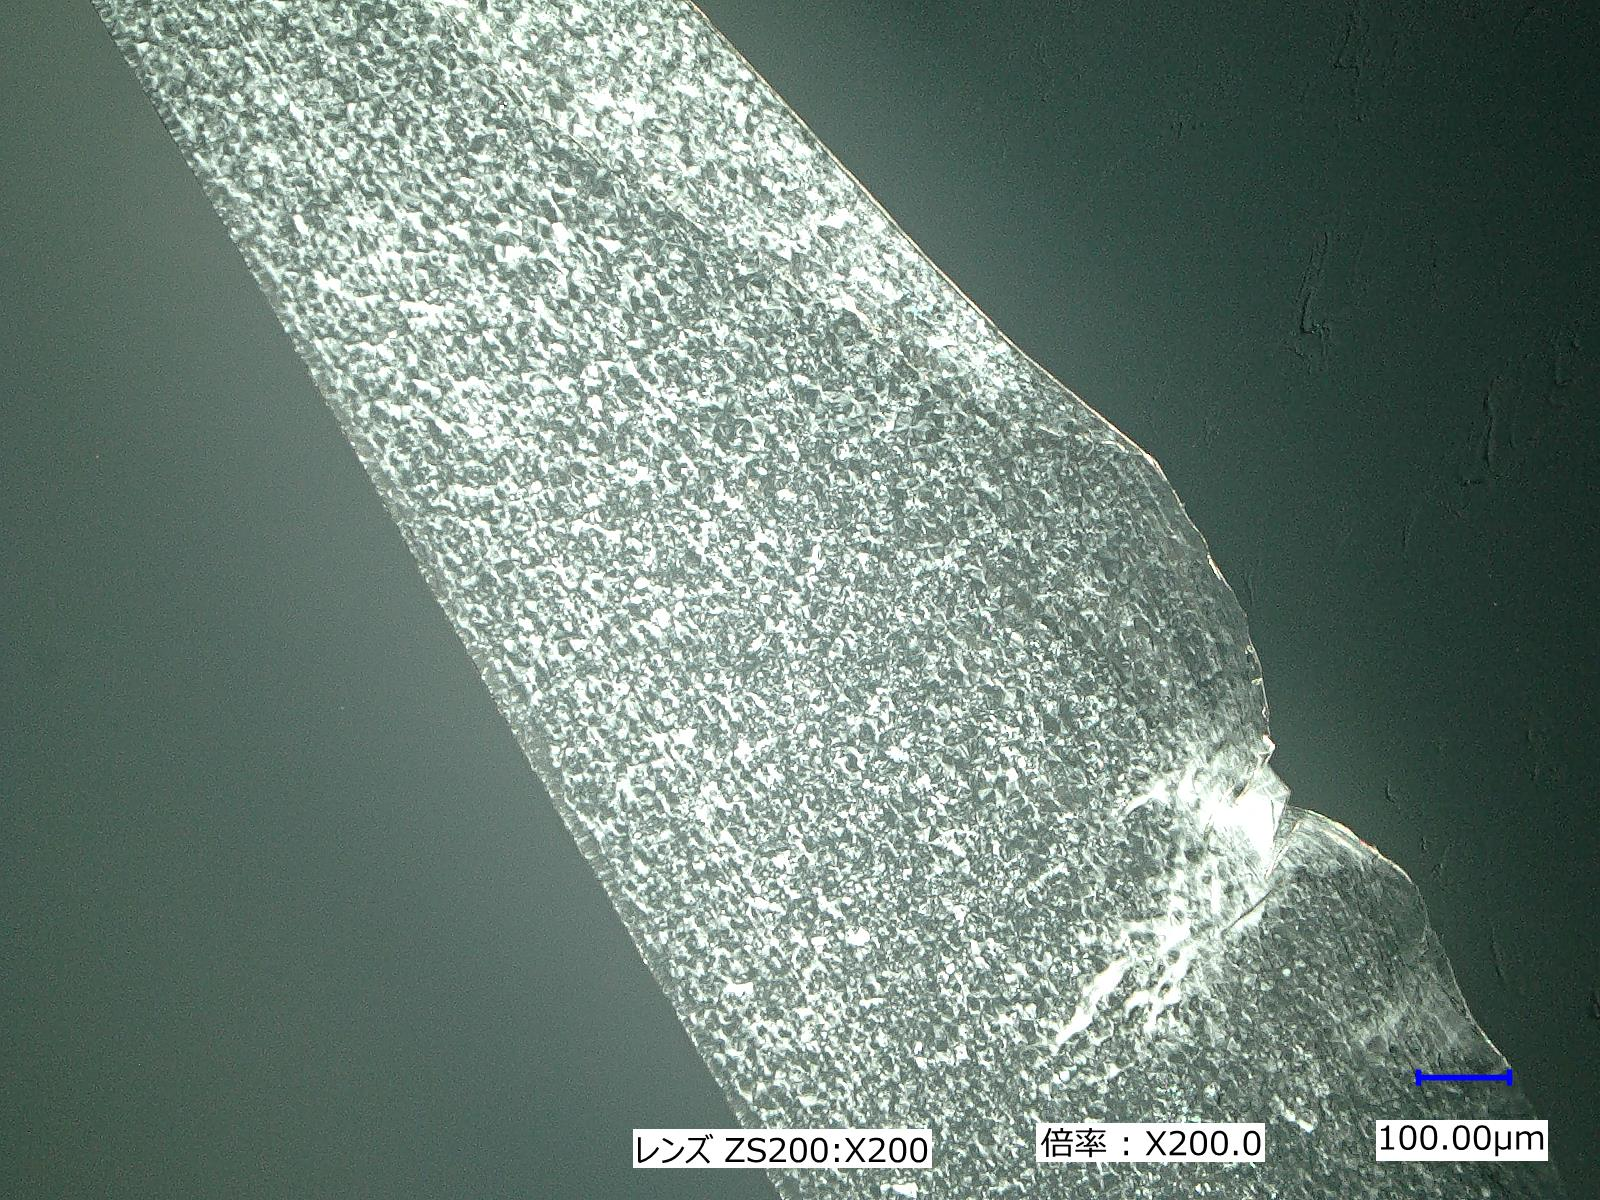
\includegraphics[keepaspectratio, scale=0.1]{Data/観察結果/rapid_cooling_200.jpg}
      \subcaption{Magnification 200x}
      \label{fig:rapid200}
    \end{minipage}
    \begin{minipage}[htbp]{0.45\linewidth}
      \centering
      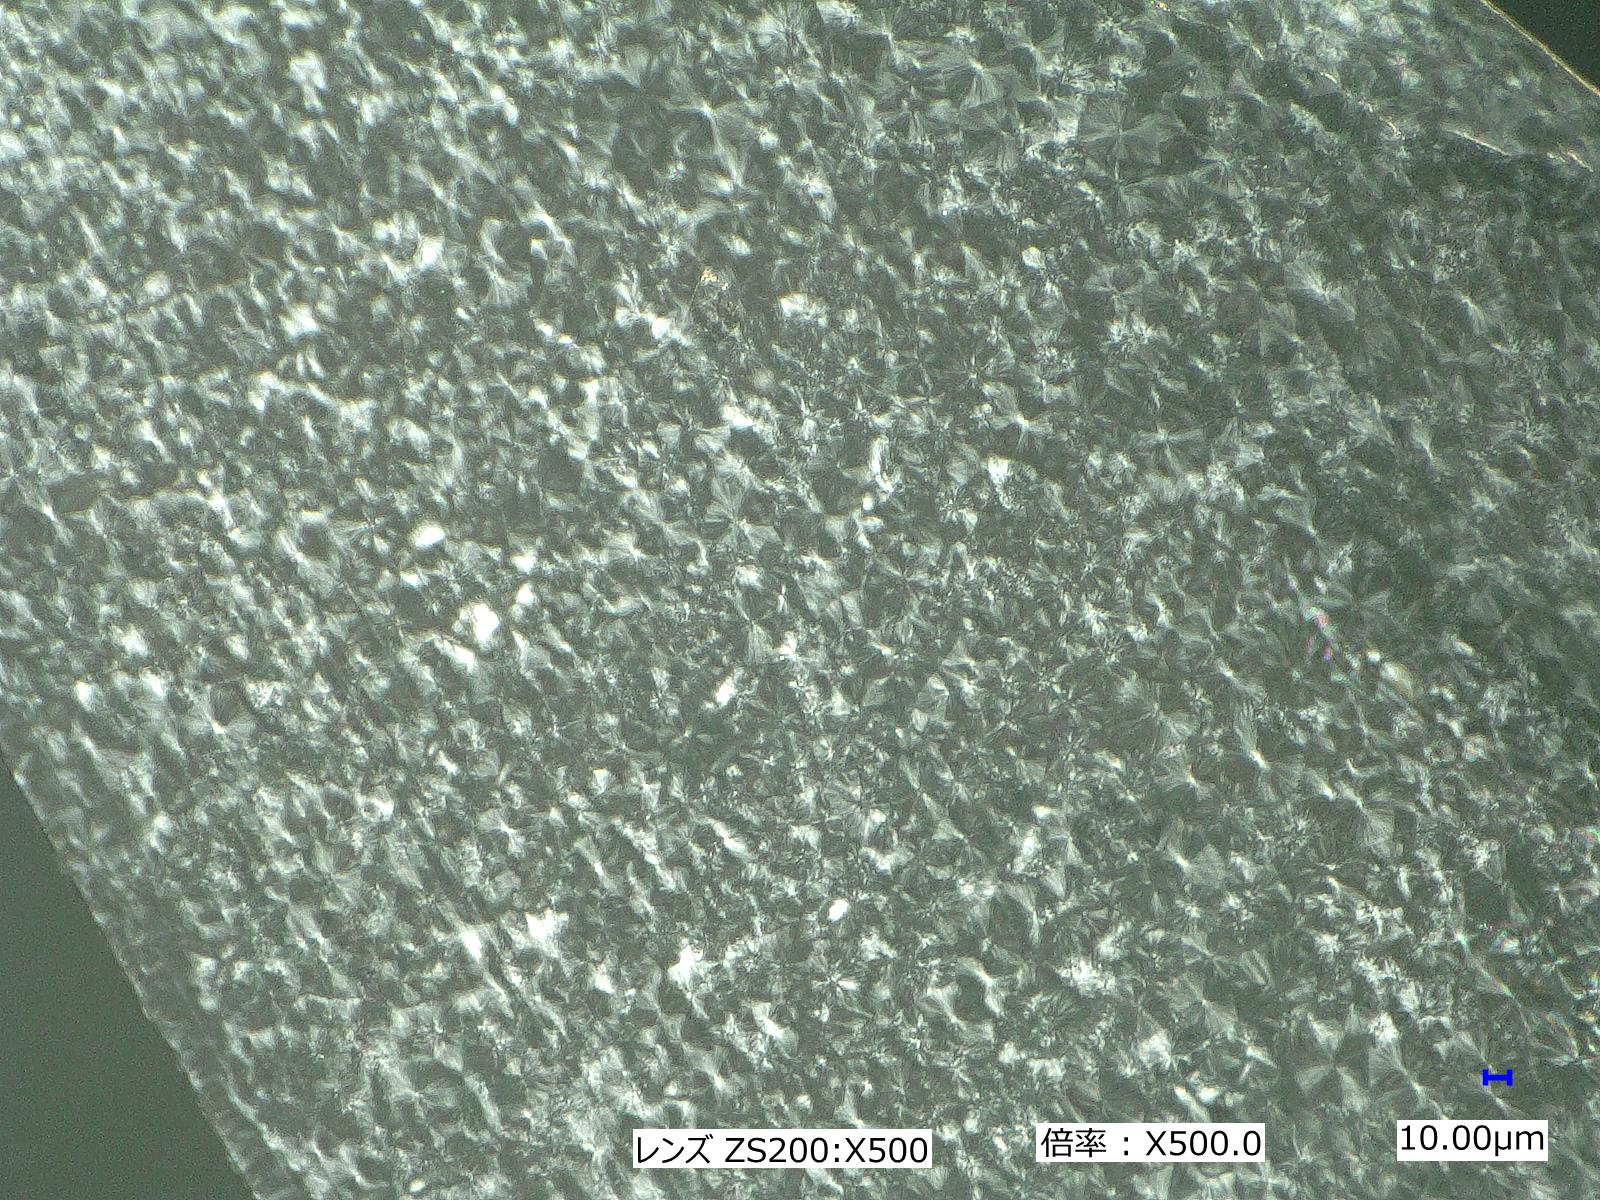
\includegraphics[keepaspectratio, scale=0.1]{Data/観察結果/rapid_cooling_500.jpg}
      \subcaption{Magnification 500x}
      \label{fig:rapid500}
    \end{minipage}
    \centering
    \caption{Rapidly cooled specimen.}
    \label{fig:rapid}
\end{figure}

\begin{figure}[htbp]
    \begin{minipage}[htbp]{0.45\linewidth}
      \centering
      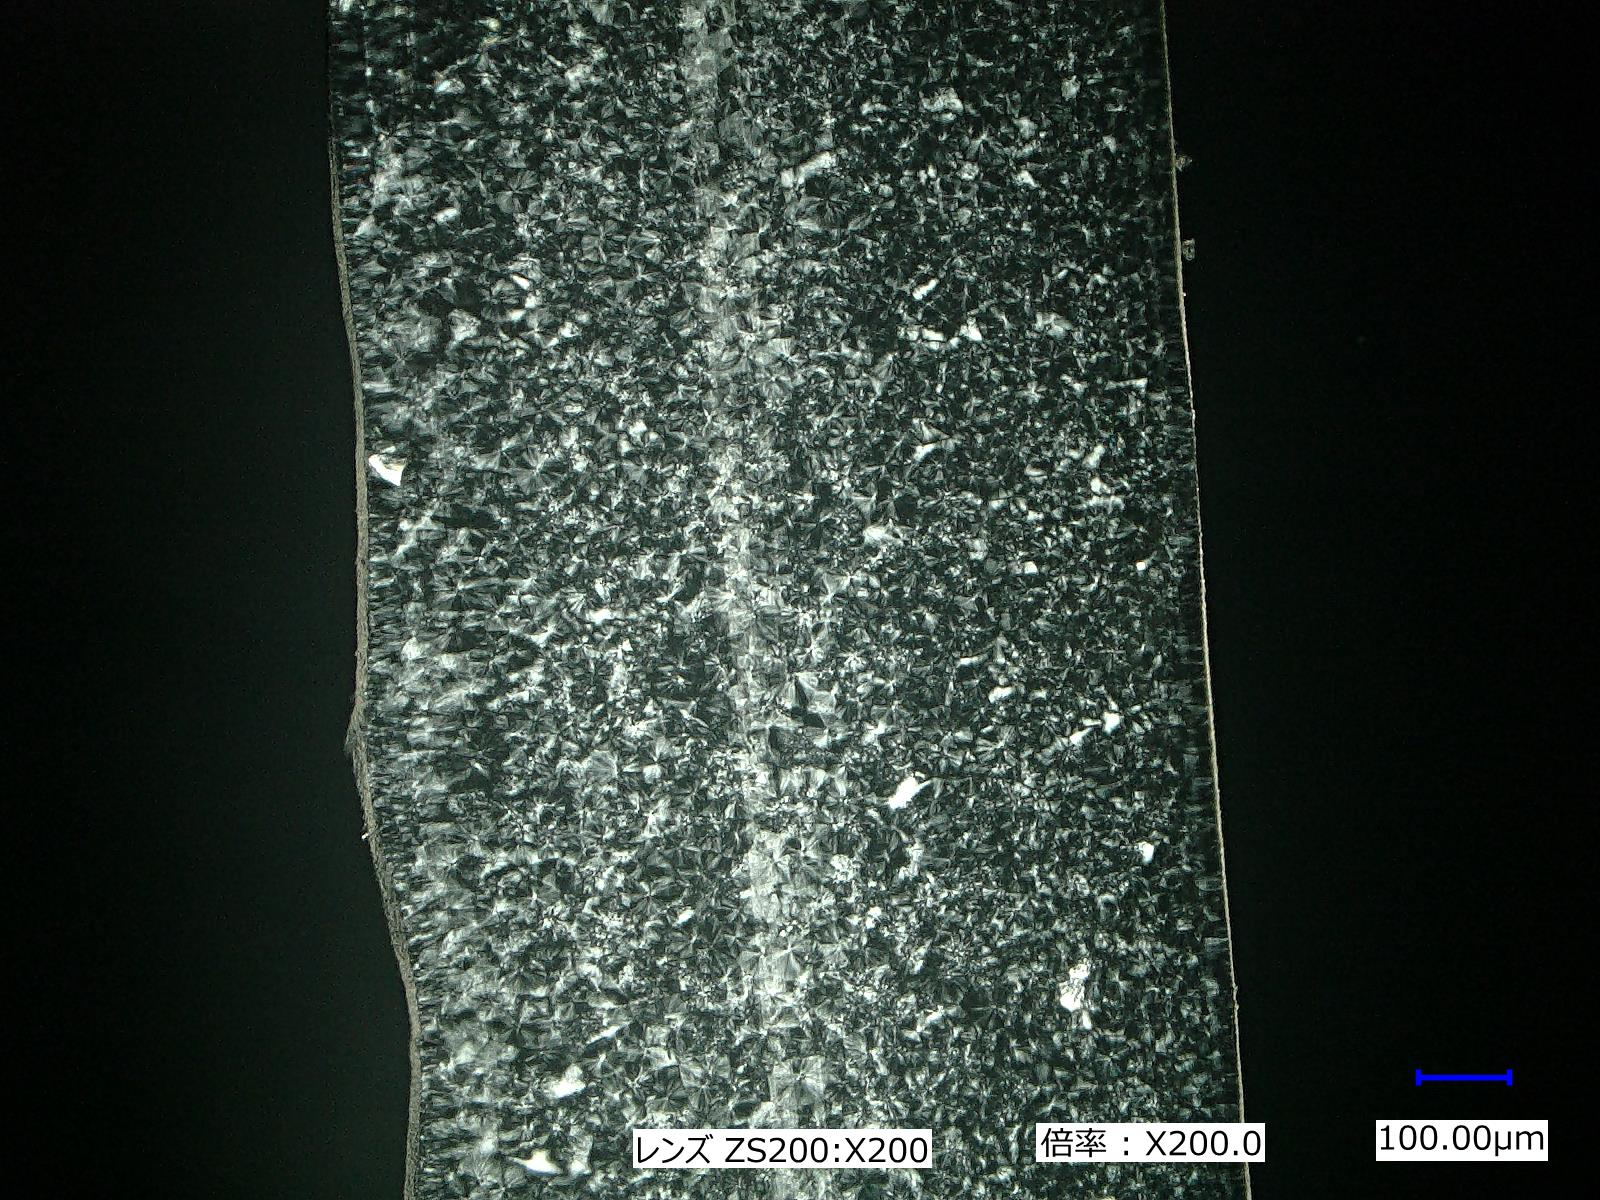
\includegraphics[keepaspectratio, scale=0.1]{Data/観察結果/65_10min_200.jpg}
      \subcaption{Magnification 200x}
      \label{fig:65度200}
    \end{minipage}
    \begin{minipage}[htbp]{0.45\linewidth}
      \centering
      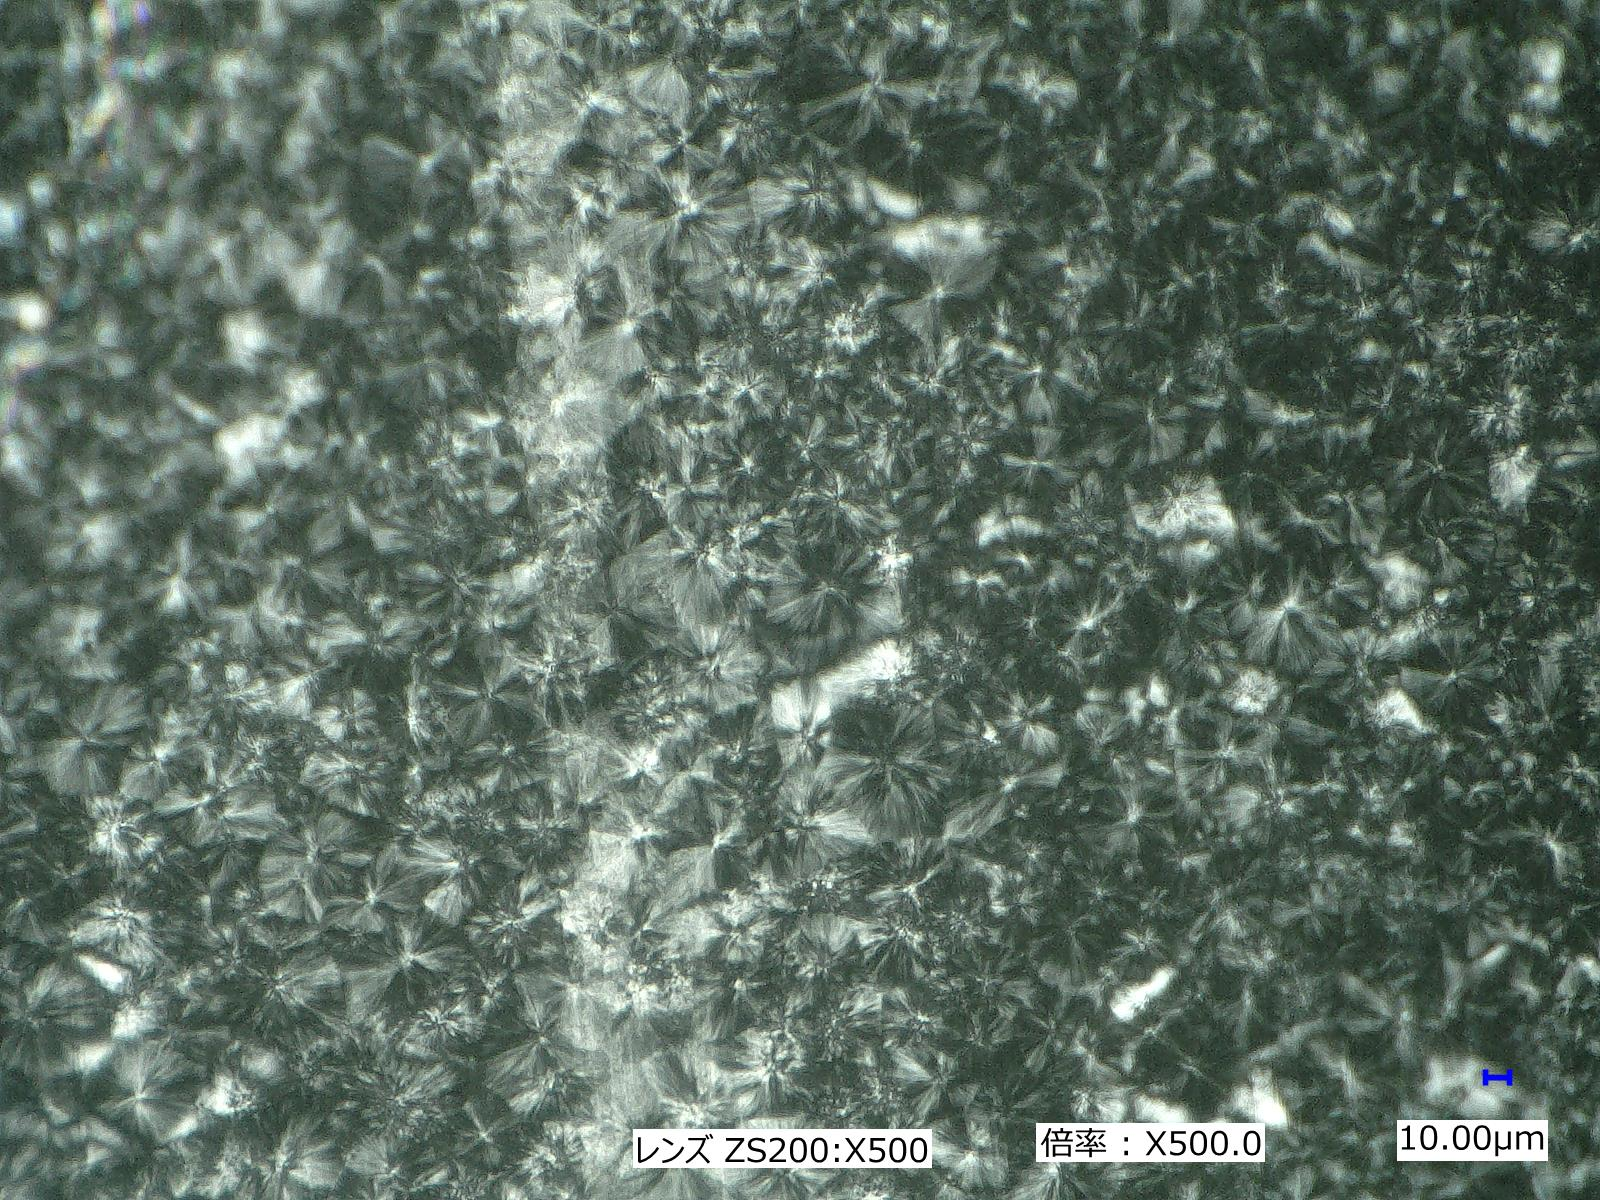
\includegraphics[keepaspectratio, scale=0.1]{Data/観察結果/65_10min_500.jpg}
      \subcaption{Magnification 500x}
      \label{fig:65度500}
    \end{minipage}
    \centering
    \caption{Specimen held at 65$^\circ$C for 10 minutes.}
    \label{fig:65度}
\end{figure}

\begin{figure}[htbp]
    \begin{minipage}[htbp]{0.45\linewidth}
      \centering
      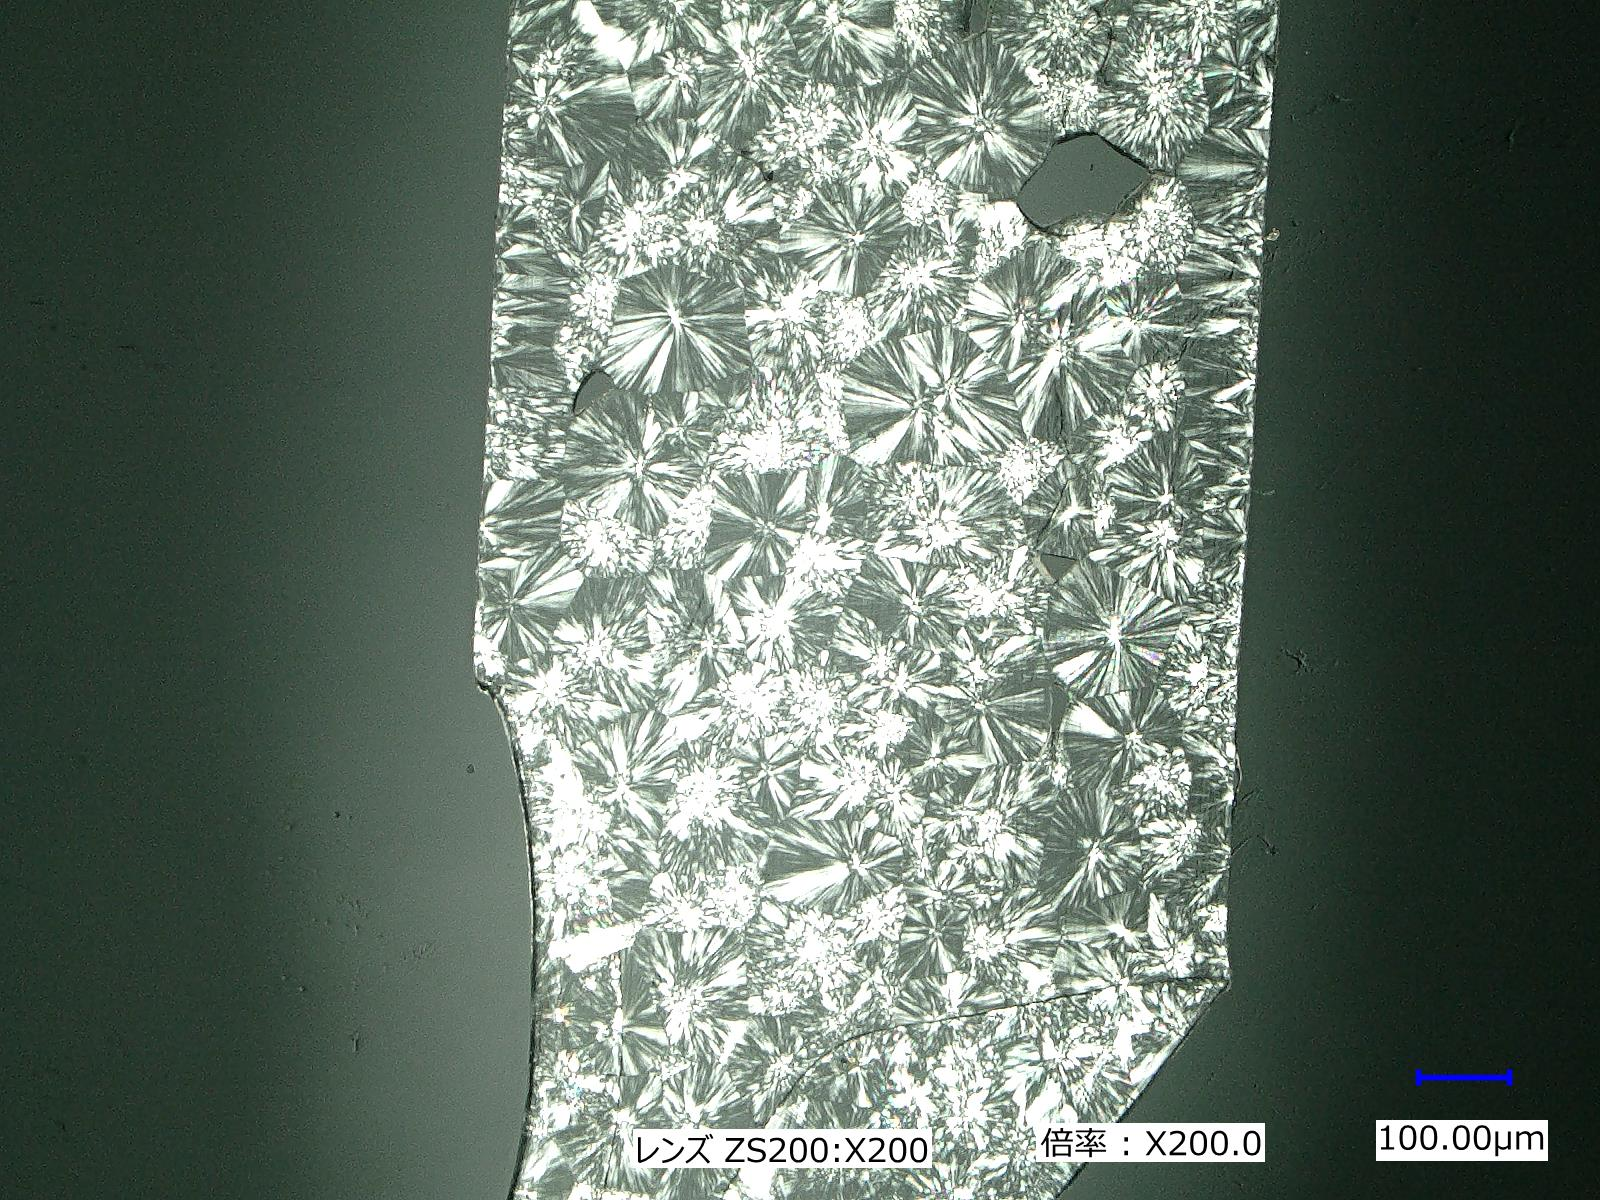
\includegraphics[keepaspectratio, scale=0.1]{Data/観察結果/120_10min_200.jpg}
      \subcaption{Magnification 200x}
      \label{fig:120度200}
    \end{minipage}
    \begin{minipage}[htbp]{0.45\linewidth}
      \centering
      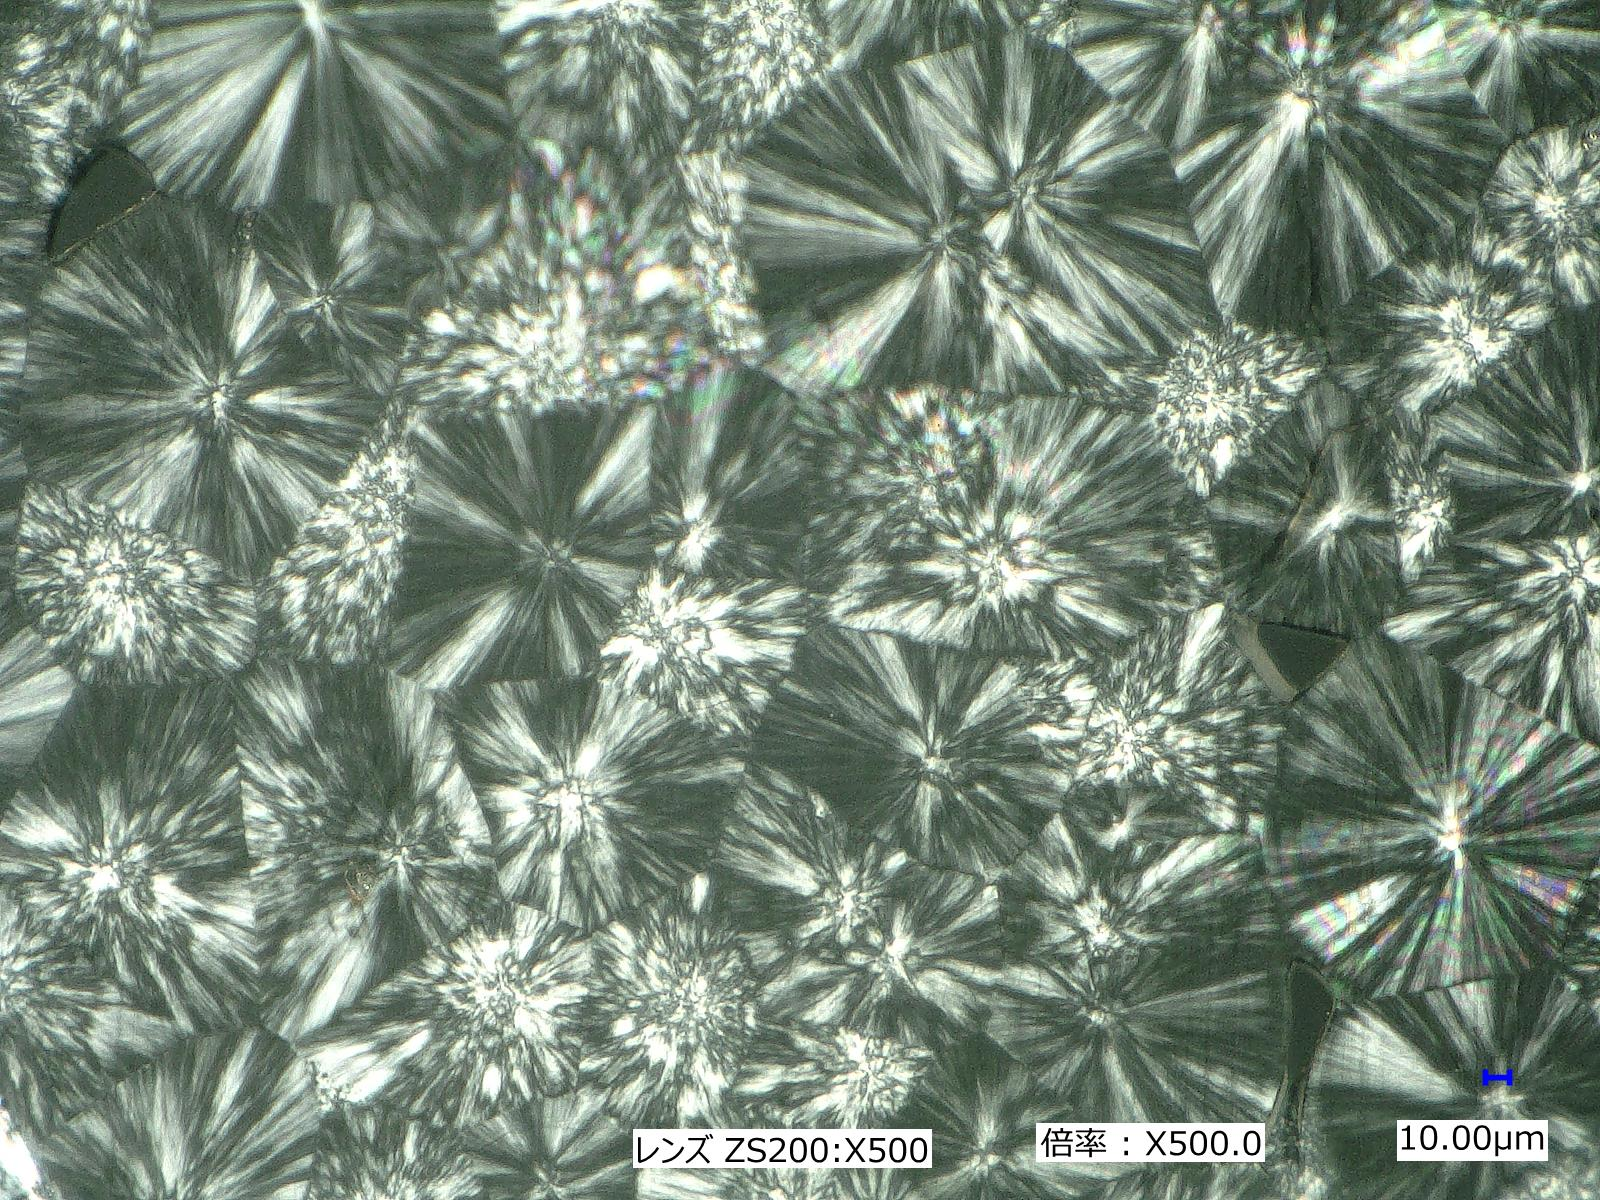
\includegraphics[keepaspectratio, scale=0.1]{Data/観察結果/120_10min_500.jpg}
      \subcaption{Magnification 500x}
      \label{fig:120度500}
    \end{minipage}
    \centering
    \caption{Specimen held at 120$^\circ$C for 10 minutes.}
    \label{fig:120度}
\end{figure}